% =====================================================================
%  WACV 2027 (Round 2) submission -- Datasets track
%
%  Built on the OFFICIAL WACV 2027 Author Kit (wacv.sty, preamble.tex and
%  ieeenat_fullname.bst are the kit's own files, copied verbatim -- do not
%  hand-edit them). Kit fetched 2026-08-12 from
%      https://wacv.thecvf.com/static/wacv-2027-author-kit-template.zip
%
%  Hard rules from the author guides:
%    * 8 pages maximum EXCLUDING references. Over-length = desk reject.
%    * Papers not using the template, or not anonymised, are rejected
%      without review.
%    * Double-blind: the [review] option below renders the author block as
%      "Anonymous WACV submission", so the \author{} content is not shown.
%      Set \wacvPaperID once CMT assigns one.
%
%  Dates (WACV 2027, Round 2): enrol 21 Aug 2026 | paper 28 Aug 2026
%
%  EVERY numeric claim is taken from reference/*.json, which are recomputed
%  from raw model output and asserted by pilot/tests/. Do not retype a
%  number from memory; run paper/check_numbers.py after editing.
% =====================================================================

\documentclass[10pt,twocolumn,letterpaper]{article}

%%%%%%%%% PAPER TYPE
\usepackage[review,datasets]{wacv}   % REVIEW version, Datasets track
% \usepackage{wacv}                  % camera-ready

\input{preamble}

\usepackage{tabularx}

\definecolor{wacvblue}{rgb}{0.21,0.49,0.74}
\usepackage[pagebackref,breaklinks,colorlinks,allcolors=wacvblue]{hyperref}

% Local layout fixes for the WACV review style. Keep wacv.sty verbatim.
\setlength{\linenumbersep}{0.18cm}
\let\makeLineNumberOdd\makeLineNumberLeft
\let\makeLineNumberEven\makeLineNumberLeft
\makeatletter
\renewenvironment{abstract}{%
   \iftoggle{wacvpagenumbers}{}{\thispagestyle{empty}}%
   \centerline{\large\bf Abstract}%
   \vspace*{6pt}\noindent%
   \it\ignorespaces%
}{%
   \vspace*{6pt}%
}
\makeatother

%%%%%%%%% PAPER ID -- update once CMT assigns one
\def\wacvPaperID{*****}
\def\confName{WACV}
\def\confYear{2027}

\newcommand{\ci}[2]{{\small$[#1,\,#2]$}}

\title{When Correctness Is the Prediction: An Evaluation Trap in
Sampling-Based Uncertainty for Handwritten Mathematics}

% Double-blind: [review] replaces this block with an anonymous byline.
\author{First Author\\
Institution1\\
{\tt\small firstauthor@i1.org}
\and
Second Author\\
Institution2\\
{\tt\small secondauthor@i2.org}
}

\begin{document}
\maketitle

\begin{abstract}
Repeated sampling provides a cheap, label-free uncertainty signal through
model self-disagreement. We evaluate it on handwritten mathematics and find
a useful transcription signal, no grading signal, and an evaluation artifact
that can manufacture an apparent effect. Against the frozen transcription
scorer, entropy reaches AUROC $0.835$, replicated at $0.828$ on a second model
family. It survives parser and ceiling controls and outperforms token
confidence and simpler summaries of the same samples. When all five samples
disagree, the scorer marks $57$ of $61$ items incorrect. For grading, however,
entropy is indistinguishable from chance (AUROC $0.520$).

Stratifying grading by its ground-truth label appears to recover AUROC
$0.801$--$0.854$ across three model families, but this effect is arithmetic.
Within a fixed-label stratum, correctness is the same binary column as the
model verdict, so uncertainty computed from those verdicts predicts
correctness almost by construction; a signal-free biased coin outscores every
model evaluated here. Transcription does not undergo this fixed-label
collapse. Finally, an exploratory single-reader audit of all $104$ items the
scorer marks incorrect attributes approximately three-quarters to the scoring
pipeline rather than to the model. Sampling disagreement can therefore
support transcription deferral, but its evaluation must test whether the
target construction or scorer creates the apparent signal.
\end{abstract}

% =====================================================================
\section{Introduction}
% ~1 page. FERMAT's own paper uses narrative prose and NO bulleted
% contributions list; matching that is the safer choice for this venue.
%
% Argument to make, in order:
%   1. Automated marking of handwritten work is a real application, and it
%      fails silently -- a wrong transcription looks exactly like a right
%      one. So knowing WHEN to defer matters more than raw accuracy.
%   2. Sampling-based uncertainty is the obvious candidate: no training,
%      no labels, works on a closed model.
%   3. But whether it works is an empirical question, and -- our point --
%      the headline number is easy to get wrong in both directions.
%   4. State the two directions concretely (pooling hides a real effect;
%      degeneracy manufactures a fake one). This is the contribution.
%   5. Say plainly this is an evaluation paper, not a method paper.
Automated marking of handwritten mathematics fails silently. When a model
misreads $4.9$ as $49$, the resulting transcription is as fluent, as
confident and as well-formed as a correct one, and nothing in the output
distinguishes the two. In a deployment where that output contributes to a
grade, determining \emph{when} to route a page to a human reviewer is more
valuable than a marginal gain in average accuracy, and unlike accuracy it
is directly actionable.

Repeated sampling, combined with a measure of the resulting
self-disagreement, is the natural candidate for such a signal. Our
output-only score requires no task-specific training, labelled
calibration data or access to model weights, and therefore applies to
closed models served behind an API. It is motivated by self-consistency
and semantic entropy~\cite{selfconsistency,semanticentropy}; whether it is
effective here remains an empirical question. We address that question on
FERMAT~\cite{fermat}, a benchmark built from textbook and competitive-exam
solutions that are systematically perturbed and then manually transcribed
and photographed. Its perturbations include both error-inducing and
correctness-preserving changes.

Effectiveness proves to be task-dependent, and, more importantly for
evaluation practice, the headline figure is easy to misestimate in either
direction. On transcription the association with the frozen scorer survives
our parser and ceiling controls. On grading it is absent. Between these two findings lies
a methodological trap. Confronted with a model whose grading verdict is
heavily biased toward a single answer, the natural response is to
stratify by the ground-truth label. Doing so appears to recover a
substantial effect that replicates across three independently trained
model families. That effect is an artifact: within a stratum in which the
true label is constant, ``was the model correct'' is arithmetically the
same column as ``what did the model answer'', so an uncertainty measure
computed from those answers predicts correctness almost by construction.
Consequently, a signal-free biased coin outscores every model evaluated
here. Notably, none of the usual safeguards detected the problem. The
pre-registered threshold did not, since the null distribution clears it;
statistical power did not, since both strata were adequately powered; and
replication did not, since it reproduced the artifact three times.

A second and more easily overlooked failure underlies both arms. The
automatic scorer that assigns correctness is itself unreliable. An
exploratory single-reader audit of every item it marked incorrect finds that
approximately three-quarters of those verdicts are attributable to the
scoring pipeline rather than to the model, while targeted checks of items it
marked correct reveal unearned passes in the opposite direction. We report
sensitivity bounds under explicit recoding assumptions, not corrected
population estimates.

This is an evaluation paper rather than a method paper. We propose no new
uncertainty estimator. Instead, we establish where a standard estimator is
effective, where it is not, and two distinct mechanisms by which an
evaluation of it can yield a confident figure that carries no information.

% =====================================================================
\section{Related Work}
% ~0.75 page. FERMAT's paper uses unnumbered thematic paragraphs rather
% than subsections -- follow that.
%
% \paragraph{Sampling-based uncertainty.} semantic entropy and its
%   variants; self-consistency; what is inherited and what is not (we use
%   exact-match clustering over an extracted answer span, not NLI).
% \paragraph{Selective prediction and abstention.} risk--coverage, AURC,
%   conformal methods; we report AURC 0.410 against a 0.607 random-deferral
%   baseline.
% \paragraph{VLMs on handwritten and mathematical content.} FERMAT,
%   ErrorRadar, ScratchMath; what they measure and what they omit.
% \paragraph{Evaluation pitfalls.} Simpson's-paradox-style aggregation,
%   class imbalance, and metric artifacts. This is where our contribution
%   is positioned -- find the closest prior work and be honest about it.
\paragraph{Sampling-based uncertainty.}
Repeated sampling turns a generator into an ensemble, and disagreement
among the samples is used as a confidence signal. Self-consistency
aggregates sampled chains by majority vote and was introduced primarily
as an accuracy-improving decoding method, although its vote distribution
can also provide an uncertainty estimate~\cite{selfconsistency}. Semantic
entropy makes uncertainty explicit by aggregating likelihoods within
bidirectional-entailment clusters and taking the entropy over the
resulting meanings~\cite{semanticentropy}. Our estimator keeps the
resampling and the entropy but replaces both likelihood weighting and
semantic grouping with empirical frequencies over exact-match clusters of
an \emph{extracted answer span}. That choice is not an oversight. On these
data, an NLI-plus-union-find implementation merged opposed clusters through a
single false-positive transitive link and degraded as $K$ grew, so the
simpler rule is the one that survives (\S\ref{sec:limitations}). A
separate line asks the model to report its own confidence, either as a
probability of being correct~\cite{kadavath} or in words; we test the
verbalized form as a baseline and it carries no signal on the arm we lead
with (\S\ref{sec:q2}).

\paragraph{Selective prediction and abstention.}
The decision this signal supports is deferral, not correction, which
places the work in selective prediction: a model may abstain, and the
question is the risk--coverage trade-off it achieves~
\cite{selectiveclassification}. We summarize this trade-off with AURC
against a random-deferral baseline and additionally report coverage at a
target risk. In vision--language reasoning, ReCoVERR reduces unnecessary
abstention on A-OKVQA and VQAv2~\cite{recoverr}. More directly for OCR,
latent-representation probes have been used to abstain from VLM-generated
OCR errors~\cite{ocrabstentionprobes}, and uncertainty-aware OCR has been
trained to mark unreliable spans in degraded
documents~\cite{uncertaintyawareocr}.
Our setting instead asks whether output-only resampling supports selective
dense transcription of handwritten mathematics. We score against the
page-faithful perturbed target, so ``correct'' means faithful to what is
written on the page, not necessarily mathematically true.

\paragraph{Vision--language models on handwritten and mathematical content.}
MathVista scores answer accuracy across diverse visual contexts, including
natural images, diagrams, charts and scientific figures~\cite{mathvista}.
Document OCR systems such as Nougat instead map pages to source-derived
markup and compare against a reference, while noting both reference
artifacts and rendering-equivalent formulae~\cite{nougat}.
FERMAT~\cite{fermat}, the benchmark used here, begins with textbook and
competitive-exam solutions, applies controlled perturbations, and has
annotators hand-copy and photograph the resulting pages. It supplies both
the original correct solution and the page-faithful perturbed version;
about $15\%$ of the perturbations preserve correctness. ErrorRadar
evaluates first-error localization and categorization~\cite{errorradar},
whereas ScratchMath evaluates error-cause explanation and
classification on authentic student scratchwork~\cite{scratchmath}.
Neither includes an error-free student-response class, although both
include correct reference solutions. Thus all three concern the diagnosis
of erroneous or perturbed work, but none benchmarks calibrated uncertainty
or selective deferral after visual transcription. On real handwritten
mathematics exams, GPT-4o grading remains below the reliability needed for
deployment~\cite{gpt4handwrittengrading}; a separate university study
reports substantial answer-extraction difficulty and confidence
false-positive rates that leave human verification
necessary~\cite{asaghandwritten}.

\paragraph{Evaluation artifacts.}
Our central negative result is that a metric can manufacture a signal
from nothing, and similar failures have appeared in prior work.
Some reported emergent abilities can arise from discontinuous metrics
rather than model behaviour~\cite{mirage}. Our case is narrower and, we think,
sharper: within a stratum where the true label is constant, correctness
becomes the same column as the model's own verdict, so a signal-free
biased coin outscores every model we tested (\S\ref{sec:trap}). The
scoring machinery is a second source of artifacts. Process-supervised
reward models have been trained to score individual steps of mathematical
solutions~\cite{verifystepbystep}. Math-specific evaluations of LLM judges
also find that they can favour stronger candidate models even when their
answers are wrong and can be persuaded to inflate incorrect
solutions~\cite{mathllmjudges,trickthegrader}. We observe a different
failure mode in one tested judge: on a perturbed-answer benchmark, it
reconstructed the mathematically correct answer and graded against
\emph{that} rather than against the reference it was given
(\S\ref{sec:limitations}).

% =====================================================================
\section{Setup}
\label{sec:setup}

\paragraph{Data.}
FERMAT~\cite{fermat} contains $2{,}244$ photographed handwritten
solutions to middle- and high-school problems. The dataset authors apply
controlled perturbations to textbook and competitive-exam solutions, and
annotators manually transcribe and photograph the results. Each image
contains a complete question and solution. Of the $2{,}244$ pages, $340$
($15.2\%$) have only superficial, correctness-preserving modifications;
we call these items error-free. That property is load-bearing for this
paper:
\S\ref{sec:q5} shows the analysis in \S\ref{sec:q3} is impossible on
datasets that lack it. Unless stated otherwise we use a balanced $n=300$
sample ($150$ with an error, $150$ without), drawn once with a fixed seed.

\paragraph{Tasks.}
We evaluate two distinct tasks on the same images.
\emph{Perception} asks the model to
``explicitly perform OCR on the handwritten text and extract the content
in \LaTeX{} format''; it is correct when the extracted final answer
matches the released page-faithful \texttt{pert\_a} field after
canonicalisation.
\emph{Reasoning} asks it to ``analyze the Answer to determine whether
there is any error'' and emit a binary judgement; it is correct when that
judgement matches \texttt{has\_error}. Neither released field is provided
directly as text to the model.

\paragraph{Uncertainty measure.}
For each item we draw $K=5$ samples at temperature $0.7$, reduce each to
a canonical label, and take the Shannon entropy of the resulting cluster
distribution, $H=-\sum_i p_i \ln p_i$. $H=0$ when all samples agree and
$H=\ln K$ when all differ. We deliberately use exact-match clustering
over an \emph{extracted answer span} rather than semantic clustering of
whole derivations; \S\ref{sec:limitations} records why.

\paragraph{Models.}
Qwen2.5-VL at 3B and 7B~\cite{qwen25vl}, Pixtral-12B~\cite{pixtral},
LLaVA-NeXT-7B and InternVL3-8B, comprising four independently trained
families, all run in bfloat16.

\paragraph{Statistics.}
Every AUROC carries a $95\%$ bootstrap interval over $10{,}000$
item-level resamples. Comparisons between conditions use a \emph{paired}
bootstrap over the same resampled items rather than checking whether two
marginal intervals overlap. Before any run we registered a minimum
minority-class size of $30$ and, for the stratified reasoning hypothesis,
an AUROC threshold of $0.70$; verdicts below are assigned by a pure
function of those thresholds, not by inspection.

\paragraph{Artifacts.}
The anonymous supplementary artifact provides the evaluation code and tests,
exact prompt hashes, a hash-only manifest for the $300$-item sample, and an
authenticated reconstruction check against a pinned FERMAT revision. Because
FERMAT is gated, the public artifact excludes its page images, released text,
and model generations derived from those pages; authorized users can
reconstruct and verify the sample without redistributing those fields.

% =====================================================================
\section{Results}
% ~3 pages. Organised as questions, following FERMAT's Section 5.

\subsection{Does self-disagreement predict transcription error?}
\label{sec:q1}
Yes, and by a margin that does not depend on the model's own confidence
being poor. On the balanced $n=300$ sample, perception entropy predicts
transcription error with AUROC~$0.835$ \ci{0.787}{0.879}. The model's own
mean token log-probability reaches only $0.537$ \ci{0.469}{0.605}, an
interval that includes chance, and the paired difference is
$+0.297$ \ci{+0.214}{+0.380}, resolved. The signal is therefore not
recoverable from information the model already exposes.

Against the frozen labels, the corresponding deferral rule marks $57$ of the
$61$ items on which all five transcriptions disagree as wrong ($93.4\%$
precision, $31.3\%$ recall). Over the full risk--coverage curve this
gives AURC~$0.410$ against a $0.607$ random-deferral baseline
(Fig.~\ref{fig:riskcoverage}).
\begin{figure}[t]
  \centering
  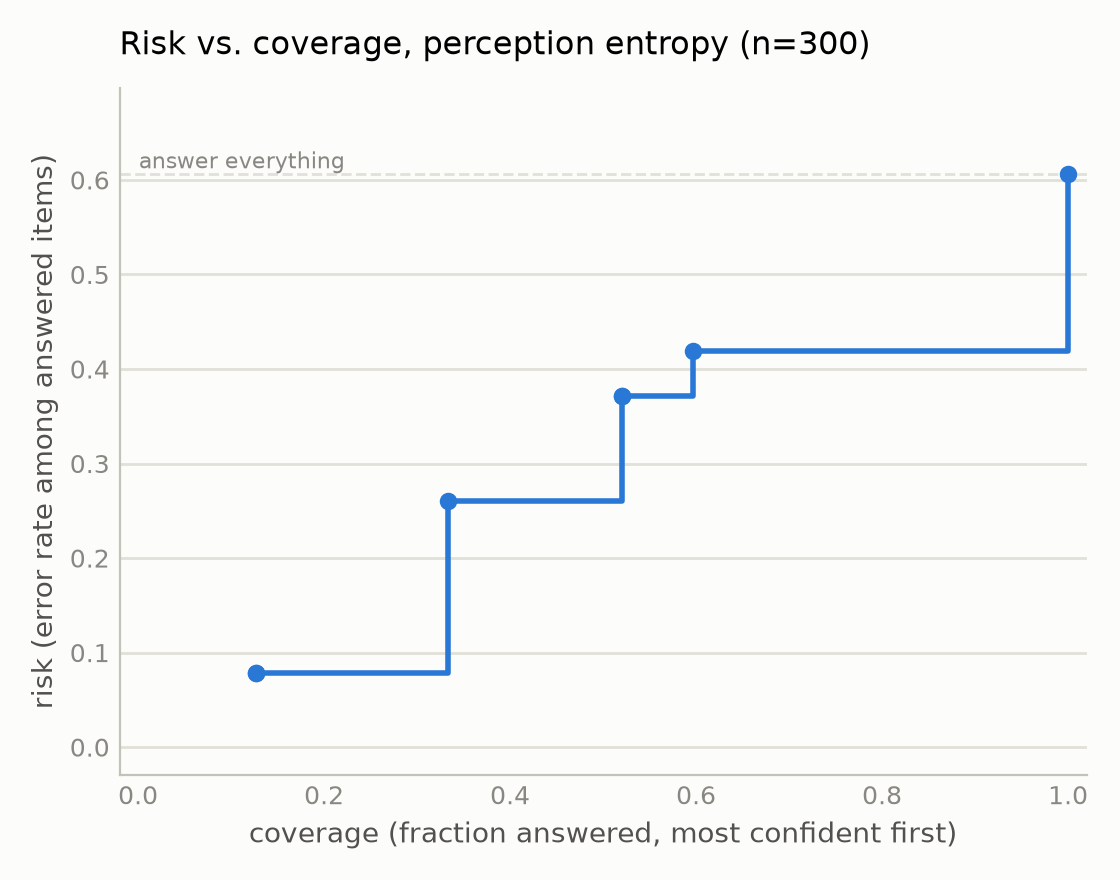
\includegraphics[width=\linewidth]{figures/risk_coverage_n300.png}
  \caption{Risk--coverage against the frozen transcription scorer for
  perception entropy, Qwen2.5-VL-3B,
  $n=300$. Deferring the highest-entropy items first traces
  AURC~$0.410$ against a $0.607$ random-deferral baseline. The curve is
  the practitioner-facing form of the result: at a $10\%$ risk target the
  rule retains $21.3\%$ coverage, and token log-probability cannot hold
  error below $40\%$ at any coverage.}
  \label{fig:riskcoverage}
\end{figure}

\subsection{Does it replicate on a second model family?}
\label{sec:q1a}
Yes. Pixtral-12B, architecturally independent of Qwen, reaches
$0.828$ \ci{0.782}{0.871} on the same $300$ images at a comparable
transcription accuracy ($41.7\%$ against $39.3\%$). The intervals overlap
along almost their whole length, so the two are not resolvably different.

More important than the point estimate is that it survives the control of
\S\ref{sec:q2}: $0.772$ \ci{0.710}{0.833} after removing both parse
failures and maximum-entropy items, with $17\%$ of items at the ceiling.
\S\ref{sec:q6} describes a fourth model that scores \emph{higher} raw and
does not survive that control, which is the reason we report the two
together.

\subsection{What does the entropy summary add?}
\label{sec:q1b}
All five samples per item support several summaries, and a natural
objection is that entropy is merely a dressed-up count of distinct
answers. Table~\ref{tab:baselines} tests that directly. The three
sample-based alternatives are computed from the \emph{same} generations at
no additional cost, so the comparison isolates the summary rather than the
sampling budget.

\begin{table}[t]
\centering\small
\setlength{\tabcolsep}{3pt}
\begin{tabularx}{\linewidth}{@{}>{\raggedright\arraybackslash}Xcc@{}}
\toprule
Signal & AUROC (95\% CI) & vs.\ entropy \\
\midrule
Sampling entropy      & 0.835 \ci{0.787}{0.879} & n/a \\
$1-$majority fraction & 0.793 \ci{0.742}{0.841} & $+0.042$ \ci{+0.011}{+0.073} \\
Distinct count        & 0.790 \ci{0.739}{0.838} & $+0.045$ \ci{+0.016}{+0.075} \\
Majority margin       & 0.779 \ci{0.727}{0.830} & $+0.055$ \ci{+0.018}{+0.092} \\
\midrule
Token log-probability & 0.537 \ci{0.469}{0.605} & $+0.297$ \ci{+0.214}{+0.380} \\
\bottomrule
\end{tabularx}
\caption{Perception baselines, Qwen2.5-VL-3B, $n=300$. The upper block
reduces the same five samples in different ways; the lower is a
model-internal signal requiring no sampling. Differences are paired
bootstraps over the same resampled items, and every one excludes zero.
Entropy's margin over the simpler summaries is small but resolved, so the
shape of the cluster distribution carries information that a count or a
majority does not. The simple summaries are related to entropy but not
redundant with it (Spearman $0.83$--$0.89$).}
\label{tab:baselines}
\end{table}

Two of these deserve comment. The majority margin separates a
three--two split from a three--one--one split, which the majority
fraction cannot, yet it remains the weakest of the three, because the
information entropy exploits resides in the full distribution rather than
in the top two clusters. Token log-probability is the only baseline here that is not a
function of the samples, and it is also the only one that fails to beat
chance; a model that is verbally or numerically confident about a page it
has misread is not detectable from its own output distribution, but is
detectable from asking it twice.
Asking the model directly fares no better. Prompted to state a confidence
from $0$ to $100$ alongside each transcription, it reports a median of
$95$ while that self-report carries no signal at all: AUROC $0.528$
\ci{0.463}{0.593}, against $0.807$ \ci{0.757}{0.854} for entropy on the
same items, a paired difference of $+0.279$ \ci{0.194}{0.359}. The
self-report is not constant, comprising $37$ distinct values spanning
$68$ to $100$. The model therefore does vary its stated confidence; it
simply varies it without tracking errors, which is the more damaging finding. Two independent
cheap-confidence baselines, token log-probability and verbalized
confidence, therefore land in the same place, and both are beaten by a
resolved margin.

The conclusion is not tied only to five samples. In a matched $K=10$ run,
entropy remains predictive against its frozen label at AUROC $0.806$
\ci{0.756}{0.854}. Holding that $K=10$ label fixed, using all ten samples
rather than the first five changes AUROC by $+0.045$
\ci{+0.005}{+0.087} and expands the observed entropy grid from $7$ to $34$
values. The main practical gain is therefore finer deferral control; this is
a sensitivity check, not a post-hoc choice of a better headline $K$.

\subsection{Does the signal survive artifact controls?}
\label{sec:q2}
A cluster-entropy AUROC can be manufactured two ways that have nothing to
do with useful uncertainty. Unparseable samples receive their own cluster
label, which both inflates entropy and correlates with being scored
wrong, so the metric could be measuring the parser. And items pinned at
the ceiling $H=\ln K$ can carry the entire ranking if that cell happens to
be uniformly incorrect, leaving a binary breakdown detector rather than a
graded signal. Table~\ref{tab:sensitivity} removes each, and both.

\begin{table}[t]
\centering\small
\begin{tabular}{lcc}
\toprule
Subset & $n$ & AUROC (95\% CI) \\
\midrule
All items                 & 300 & 0.835 \ci{0.787}{0.879} \\
Excl.\ parse failures     & 255 & 0.839 \ci{0.790}{0.886} \\
Excl.\ max-entropy items  & 239 & 0.794 \ci{0.737}{0.848} \\
Excl.\ both               & 206 & 0.796 \ci{0.736}{0.852} \\
\bottomrule
\end{tabular}
\caption{Perception entropy under artifact controls, Qwen2.5-VL-3B.
The signal is graded rather than concentrated at the ceiling: it survives
the harshest simultaneous cut with an interval excluding chance.
\S\ref{sec:q6} shows a model for which it does not.}
\label{tab:sensitivity}
\end{table}

\paragraph{Is the reported operating point a tuned one?}
The sampling temperature and the number of samples are free parameters, so
a single setting invites the objection that it was chosen after seeing the
result. We regenerated the full transcription arm over a declared grid of
three temperatures $\{0.3, 0.7, 1.0\}$ and three sample budgets
$\{3, 5, 10\}$, $9{,}000$ fresh generations under a different seed from the
frozen run, and applied the controls of Table~\ref{tab:sensitivity} to each
of the nine conditions. The signal is present in all nine: every interval
excludes chance after removing both parse failures and ceiling-entropy
items. At the reported protocol the regenerated figure is $0.830$
\ci{0.784}{0.874}, reproducing the locked $0.835$ \ci{0.787}{0.879} on
independent draws.

The grid also supplies a caution against reading raw numbers across
protocols. Uncontrolled AUROC increases with temperature, reaching $0.892$
\ci{0.857}{0.924} at $T{=}1.0, K{=}5$, which would appear to argue for
hotter sampling. It does not survive the controls: the same condition falls
to $0.722$ \ci{0.621}{0.815}, against $0.741$ \ci{0.684}{0.795} at
$T{=}0.3$, and the two intervals overlap. The correction grows with
temperature because the artifacts do; the parse-failure rate rises from
$0.5\%$ to $12.7\%$, transcription accuracy falls, and at $T{=}1.0$ the
controls remove roughly two thirds of the items. The apparent gain is the
artifact the controls exist to remove, not a better uncertainty estimate,
and we therefore report no temperature effect.

\subsection{Does the same signal work for grading?}
\label{sec:q3}
No. On the same $300$ images, reasoning entropy predicts grading error
with AUROC~$0.520$ \ci{0.458}{0.582}, an interval containing chance. The
balanced sample matters: the model answers ``there is an error'' for the
large majority of inputs, and on an unbalanced set that bias alone would
score well.

This is the honest reasoning result, and \S\ref{sec:trap} is an account of
why we did not initially believe it.

\subsection{The trap: stratifying by the label being predicted}
\label{sec:trap}
% The methodological contribution. Written as a retraction because that is
% what it is, and because the failure is more instructive than a warning
% stated in the abstract would be.
A model with a strong answer bias makes a pooled statistic hard to read,
and the natural response is to stratify by ground truth and analyse each
label separately. Doing so appears to recover a large effect from the null
above. Within the \texttt{has\_error}=1 stratum, entropy predicts grading
error at $0.801$ \ci{0.751}{0.846}; within the \texttt{has\_error}=0
(correctness-preserving) stratum it predicts in the opposite direction at
$0.280$ \ci{0.200}{0.366}. Both
strata are adequately powered, both intervals exclude chance, the sign
reversal has an appealing mechanistic story, and the effect reproduces
across three independently trained model families
(Table~\ref{tab:trap}). We reported this as our main finding.

It is an artifact, for a reason that applies to any binary-decision task
evaluated this way. \textbf{Within a stratum where every item shares the
same true label, ``was the model correct'' is not a separate fact from
``what did the model answer''; the two are the same column.} On our
$7$B run they agree on $100\%$ of items, and the AUROC against correctness
is numerically identical to the AUROC against the model's own verdict.
Entropy is computed from precisely the votes that produce that verdict, so
the measurement is near-circular. The sign reversal follows by the same
identity: in the \texttt{has\_error}=0 stratum correctness is the exact
\emph{complement} of the verdict, so anything correlating with the verdict
must invert. The two stratum AUROCs sum to $1$.

\begin{table}[t]
\centering\small
\begin{tabularx}{\linewidth}{@{}>{\raggedright\arraybackslash}Xccc@{}}
\toprule
Model & Observed & Bias-only null & Collapse \\
\midrule
Qwen2.5-VL-3B & 0.854 & 0.901 \ci{0.849}{0.932} & 99.8\% \\
Qwen2.5-VL-7B & 0.801 & 0.868 \ci{0.821}{0.903} & 100.0\% \\
LLaVA-NeXT-7B & 0.775 & 0.831 \ci{0.770}{0.874} & 97.2\% \\
\bottomrule
\end{tabularx}
\caption{The apparent replication, against a null with no item-level
signal at all: a model answering ``error'' with fixed probability per
sample, so its entropy is pure sampling noise. The null \emph{exceeds}
every observed value. ``Collapse'' is the fraction of items on which
correctness and the model's own verdict are the same label. Even the
null's $2.5$th percentile clears the $0.70$ threshold we had registered in
advance as confirming the hypothesis, so that threshold could never have
separated signal from arithmetic.}
\label{tab:trap}
\end{table}

The effect is not specific to the frozen $K=5$ protocol. A grid over
$K\in\{3,5,7,9,15\}$ and response bias $p=0.05,\ldots,0.95$ shows the
same pattern: the artifact vanishes at $p=0.5$, grows as the response
bias increases, and is removed by balanced pooling.

The mechanism is arithmetic rather than behavioural. On the
error-containing response subset, the majority vote is wrong only when
most samples differ from the model's default, and those minority votes
are exactly what raise entropy.
Nothing about the model's competence is required for the association to
appear.

Three things would have caught this earlier, and none of them is
specialised. Comparing against a signal-free null rather than against
chance, since $0.5$ is the wrong reference point for a stratified
statistic. Checking whether the correctness label is a relabelling of the
prediction before computing anything. And treating a pre-registered
threshold as necessary but not sufficient, since ours was cleared by the
null.

\subsection{Why transcription is not affected}
\label{sec:whyperception}
Both tasks have ground truth; what differs is how many values it can take.
Grading truth is binary, so stratifying by it makes the truth
\emph{constant} within each group, and correctness reduces to
$\text{correct} = (\text{majority vote} = \text{that constant})$, a
function of the vote, which is precisely what entropy summarises.
Transcription truth is a mathematical expression drawn from an effectively
unbounded set. Five samples can agree perfectly on
$\frac{5}{2(x-1)}$ and still be wrong because the reference was
$\frac{5}{2(x+1)}$, so agreement carries no guarantee of correctness. In
the data, $38$ items are unanimous and $3$ of those are wrong, while $4$
items at maximum entropy are right; correct and incorrect items occur at
both ends of the entropy range.

It is worth being precise about which ingredient does the damage. The
collapse is caused by \emph{stratifying} rather than by the label type;
grouping transcription items by their exact reference answer would
collapse in exactly the same manner. Low cardinality is what makes stratification both
tempting and total: with a binary label it is the natural response to class
imbalance, and it yields precisely two single-label groups. With
hundreds of distinct answers nobody would stratify, because the groups
would have one member each. The trap is therefore specific to
binary-decision tasks, which is where it is most likely to be walked into.

Consistent with this, \S\ref{sec:q1b} shows transcription entropy
outperforming simpler summaries of the same votes; a measure that were
merely counting minority votes could not.

\subsection{What happens on a second dataset?}
\label{sec:q5}
The analysis in \S\ref{sec:q3} requires both error-containing and
error-free evaluated solutions. ErrorRadar~\cite{errorradar} supplies
correct and incorrect solutions as paired fields, but every evaluated
candidate solution contains an annotated error.
ScratchMath~\cite{scratchmath} includes correct answer and solution fields,
but every evaluated student answer is labelled incorrect. Neither
therefore supplies an error-free response stratum for our binary grading protocol, so neither
can support a balanced replication or exhibit the inversion.

On ScratchMath, which is the only one of the two with handwriting to
grade, the measurement fails for a second and more instructive reason.
Grading accuracy reads $96.0\%$, but every evaluated student answer is
erroneous and the model answers ``error'' for $90\%$ of them, so it scores
well by construction. In $24\%$ of readings ($120/500$) the model explicitly
states it cannot read the image, and in $82\%$ of those ($98/120$) it
answers ``error'' regardless. Excluding those readings does not clean the
estimate: all four misgraded items lie among them, so the retained subset
has no minority class and the AUROC is undefined rather than improved.
We therefore report this setting as \emph{gated}: not a negative result
about uncertainty, but a statement that the pair cannot test it.

\subsection{When does a high score mean nothing?}
\label{sec:q6}
InternVL3-8B attains the highest raw perception AUROC in our study,
$0.915$ \ci{0.880}{0.944}, on a transcription accuracy of $21.0\%$,
approximately half that of the model in \S\ref{sec:q1}. Independently recomputing
every derived column from raw output reproduces the stored values
exactly, so this is model behaviour rather than a scoring defect. Under
the control of \S\ref{sec:q2} it collapses to $0.556$ \ci{0.495}{0.614}.

The mechanism is visible in the entropy distribution: $202$ of $300$
items sit at the ceiling, and accuracy within that group is $0.99\%$
against $62.2\%$ elsewhere. The score is separating total generation
breakdown from everything else, which is a binary property of the output,
not graded uncertainty about content. Reported without the control, it
would have been the strongest number in this paper.
\begin{figure}[t]
  \centering
  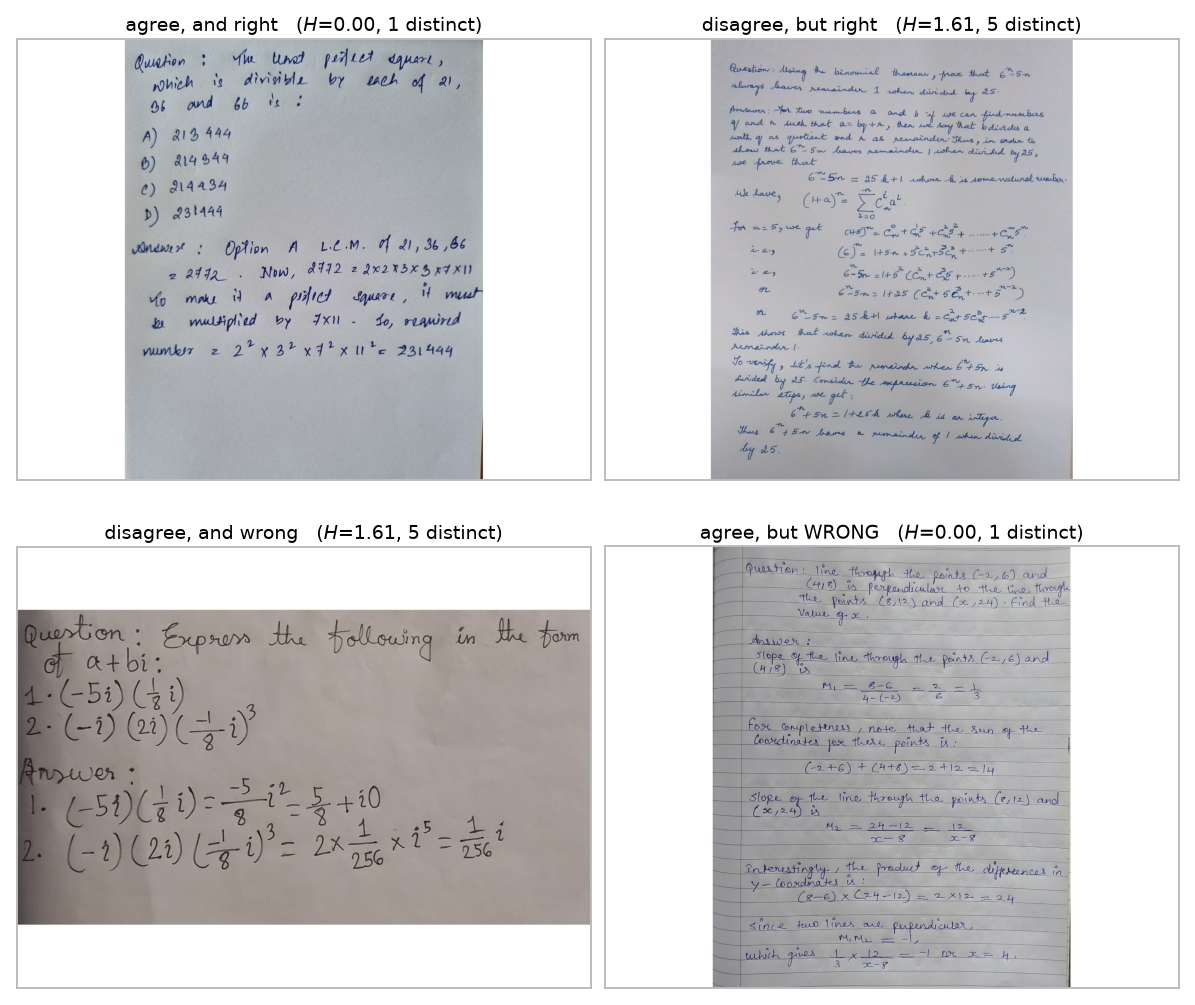
\includegraphics[width=\linewidth]{figures/four_quadrant.png}
  \caption{Four perception cases. Self-disagreement helps when wrong
  answers produce varied samples, but it is weakest when the samples mostly
  agree on the same wrong reading. The top panels were scored correct and
  the bottom panels were scored wrong; the left panels have low entropy and
  the right panels have high entropy. Each panel gives its item, entropy and
  human-audit verdict.}
  \label{fig:quadrants}
\end{figure}

% =====================================================================
\section{Failure Analysis}
\label{sec:failures}
% ~0.75 page. Reading real cases; this is what the E&D track rewards and
% what a reviewer will look for beyond the tables.
%
% Established from manual inspection so far:
%   (a) the model verifies a solution's core computation and stops, it
%       does not check whether the final statement is complete
%       (unsubstituted variable), internally consistent (mismatched
%       notation), or licensed by the problem (fabricated unit);
%   (b) it pattern-matches a stated result instead of recomputing, it
%       accepted 19 x -18 x 23 = -7966 (correct: -7866);
%   (c) confidently-wrong items are structurally invisible to the method.
For an exploratory failure analysis, one reader inspected and coded every
item the frozen rule marked wrong on Qwen2.5-VL-3B, a complete census of that
bucket comprising $104$ of $104$ items, working from the handwritten pages
rather than from the extracted text. The
distribution is not what the aggregate number suggests:

\begin{center}\small
\begin{tabular}{lrr}
\toprule
coded reason & $n$ & share \\
\midrule
scoring/extraction attributable & $77$ & $74.0\%$ \\
notation misread & $22$ & $21.2\%$ \\
undecidable from the page & $4$ & $3.8\%$ \\
copied a different line & $1$ & $1.0\%$ \\
\textbf{hallucination} & $\mathbf{0}$ & $\mathbf{0\%}$ \\
\bottomrule
\end{tabular}
\end{center}

Three things follow. First, the reader assigned \textbf{zero hallucination
labels in this $104$-item bucket}; this is evidence about the audited set,
not a population-level claim that the model never hallucinates.
Second, roughly three-quarters of what the scorer calls model error is
attributable to the scoring pipeline, either through the extractor
selecting a wrong or partial span, or through normalization collapsing a
long answer onto a single symbol. Third, and this is the constraint on the method rather than on
the model, \emph{the errors that remain are not the ones entropy can
  flag}: a low-entropy wrong item is one where the samples mostly agree, so
self-disagreement has little to use, whichever way the label happens to
fall (Fig.~\ref{fig:quadrants}, bottom-left panel).

Two mechanisms recur in the coded notes and both concern the final
answer statement rather than the mathematics. The model verifies a
solution's core computation and stops, without checking whether the final
statement is complete (a variable never substituted), internally
consistent (a tuple introducing $z$ while the condition repeats $x$), or
licensed by the problem (a unit the problem never gave). And it
pattern-matches a stated result instead of recomputing it, accepting
$19 \times -18 \times 23 = -7966$ where the correct value is $-7866$.

The coding is a single reader's, which is its main weakness. We have no
second-rater agreement. We do have an intra-rater measurement: $78$ items
were coded twice in independent passes with different sheets; $47$ received
determinate labels in both passes, and $4$ of those pointed opposite ways.

% =====================================================================
\section{Limitations}
\label{sec:limitations}
The positive result rests on one dataset. It now holds on two model
families (\S\ref{sec:q1a}), but two further models could not test it: one
sits at a transcription floor of $0.8\%$, and one fails the artifact
control of \S\ref{sec:q2}. Two of four attempts producing a usable
measurement is itself worth stating, since the result requires a model
with genuine dense-OCR competence, which is not the common case among
open-weight VLMs. Of the two alternative datasets, neither supplies
error-free evaluated responses, so neither admits a balanced
error-presence sample. Moreover, by \S\ref{sec:trap}, a
\texttt{has\_error}=1 response set constitutes a single-label stratum, on
which the measurement collapses for the same reason.

We report the correction to \S\ref{sec:trap} as a finding, but it was
found late. It was not caught by the pre-registration, which set a
threshold the null clears; nor by adequate power, which both strata had;
nor by replication, which reproduced the artifact three times. Cross-model
agreement is worth less than it appears when the mechanism is arithmetic
rather than behavioural.

Our clustering is exact-match over an extracted answer span, not semantic.
Semantic clustering was attempted and abandoned: an NLI-plus-union-find
implementation merges opposed clusters through a single false-positive
transitive link and degrades at larger $K$. The reported results avoid
that path rather than depending on it being fixed.

Confidence intervals were added after the experiments were designed and
run. They corrected several conclusions but cannot supply power the
studies were not sized for. $K=5$ also gives few operating points, which
is why two-thirds of conformal calibration splits cannot reach a $30\%$
risk target.

\paragraph{The correctness label is noisy in both directions.}
Every AUROC above is measured against a frozen string-matching rule, and a
single-reader audit indicates that rule has substantial label noise. The census of
\S\ref{sec:failures} finds unearned \emph{failures}; a seeded random
audit of the items the rule marked \emph{correct} finds unearned passes
as well. Under alternative recoding assumptions applied to these audits,
transcription accuracy ranges from roughly $44$--$61\%$, and AUROC from
$0.57$--$0.73$, depending in part on whether an unearned pass is treated as
a model error or as undecidable. These are \emph{sensitivity bounds}, not
corrected population estimates: the audit sets overlap, two are targeted in
one direction, and all coding is from one reader. Table~\ref{tab:audit}
summarizes the audited sets and their sampling restrictions.

This does not erase the frozen-scorer association, and it is worth being
precise about what it does. The distinct-answers relationship and the
cross-family replication rest on the frozen rule's stored columns, which
are unchanged. What is now in question is how well that rule's labels
track human judgement. The honest statement is that \textbf{entropy
predicts frozen-scorer failures; predicting human truth is harder}, and
that the automatic scorer is least reliable exactly where answers are
long, multi-part, set-valued, or stated as prose.

\paragraph{No automatic scorer we tried was reliable on our probes, including judges.}
We evaluated four alternatives to the frozen rule. The frozen rule is
brittle in the ways above. A
span-primary variant that demotes symbolic normalization to a warning
does not eliminate the unearned passes, because where both sides extract
the same incorrect span, span matching agrees exactly as the normalizer
did; its risk flags do, however, concentrate them. A symbolic equivalence
checker is unsafe by construction on this benchmark, because the injected
errors are often units, coefficients or notation, exactly what an equivalence checker is
designed to erase. Two open math judges failed differently: one rejected
a valid probe outright, and the other returned the correct verdict on
both probes while its own justification showed it had reconstructed a
mathematically correct reference from the problem text and graded against
\emph{that} rather than against the perturbed reference it was given,
misattributing the reference's answer to the model in the process. That
last case is the more instructive: \textbf{a verdict-only check cannot
detect it}, and on a judge that emits no reasoning it would have been
recorded as a clean pass. Grading a perturbed-answer benchmark asks a
judge to compare rather than to solve; in our probes, one judge instead
attempted to reconstruct and solve the problem.

\begin{table}[t]\centering\small
\begin{tabularx}{\linewidth}{@{}>{\raggedright\arraybackslash}Xrr>{\raggedright\arraybackslash}X@{}}
\toprule
audit set & $n$ & unearned & caveat \\
\midrule
rule said wrong   & $104$ & $77$ & complete census; one coder \\
rule said correct & $100$ & $4$--$16$ & two passes disagree \\
flagged tier      & $108$ & $39$ & high-risk by construction \\
\bottomrule
\end{tabularx}
\caption{Exploratory single-reader audit of the frozen scorer.
\textbf{These rows must not be
summed or pooled.} $78$ items are shared between sets (union $234$, not
$312$), and two of the three sets can only find errors in one direction
by construction, so a pooled agreement figure would be largely
tautological. The correct-side range spans two independent passes over
disjoint random draws which disagree at $p=0.00007$. That disagreement,
rather than either endpoint, is why accuracy is reported only as a
sensitivity range.}
\label{tab:audit}
\end{table}

% =====================================================================
\section{Conclusion}
On handwritten transcription, self-disagreement across repeated samples
predicts failures of the frozen scorer: it survives the parser and ceiling
controls, beats the model's own confidence and simpler summaries of the same
samples, and marks $57$ of $61$ maximum-entropy items as wrong under that
scorer. The single-reader audit shows why this must not be equated with human
truth. On grading, the same measure carries no signal at all.

The distance between those two sentences is where the work is. Stratifying
the grading task by ground truth, an ordinary response to a biased model,
produces an effect of $0.80$--$0.85$ that is adequately powered,
resolves against chance, clears a pre-registered threshold, and replicates
across three independently trained model families. It is still an
artifact, because within a single-label stratum the correctness label is
the model's own answer under another name. A signal-free biased coin
scores higher.

We therefore recommend, for any evaluation of sampling-based uncertainty
on a binary decision task: check whether the correctness label is a
relabelling of the prediction before computing anything, and compare
against a signal-free null rather than against $0.5$. Neither is
expensive. Together they expose failures that aggregate AUROC can hide.

A third caution follows from the audit in \S\ref{sec:limitations} and
applies more broadly than to uncertainty work. On a benchmark whose
page-faithful answers may be deliberately perturbed, the scorer is part of
the experiment. In our tests, the frozen string matcher, a symbolic
equivalence checker and two open math judges failed in different ways: one
judge rejected a valid probe, while another reconstructed a mathematically
correct answer instead of comparing against the supplied reference. Where
a correctness label is itself estimated, it deserves the same careful
validation as the quantity being estimated against it.

{
    \small
    \bibliographystyle{ieeenat_fullname}
    \bibliography{refs}
}

\end{document}
